\documentclass[11pt]{article}
\usepackage{amsmath, amssymb, amsfonts,  graphicx, enumerate, float, wrapfig}
\usepackage[margin=0.5in]{geometry}
\graphicspath{{./}}
\newcommand*{\vs}{\vspace{1cm}}
\newcommand*{\next}{\noindent}
\newcommand*{\set}{\setcounter{equation}{0}}


\title{3.4 Concavity and the Second Derivative Test}
\author{Juan J. Moreno Santos}
\date{October 2023}

\begin{document}
\maketitle

\section{The graph of $f$ is shown. State the signs of $f'$ and $f''$ on the interval (0, 2)}
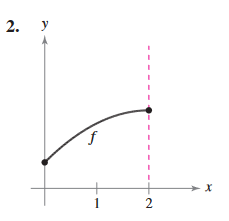
\includegraphics{2.png}\\
$f'>0$ and $f''<0$

\next
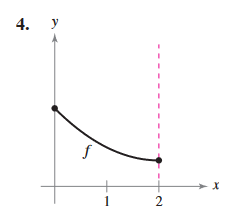
\includegraphics{4.png}\\
$f'<0$ and $f''>0$

\section{Determine the open intervals on which the graph is concave upward or concave downward.}
6.\begin{align}
    y&=-x^3+3x^2-2\\
    y'&=-3x^2+6x\\
    y''&=-6x+6
\end{align}
The graph is concave upward on $(-\infty, 1)$ and downward on $(1, \infty)$.

\vs
\next
14.\begin{align}
    \set
    y&=\frac{1}{270}(-3x^5+40x^3+135x)\\
    y'&=\frac{1}{270}(-15x^4+120x^2+135)\\
    y''&=-\frac{2}{9}x(x-2)(x+2)
\end{align}
The graph is concave upward on $(-\infty, -2)$ and $(0, 2)$, and downward on (-2, 0) and $(2. \infty)$.

\vs
\next
18.\begin{align}
    \set
    y&=x+\frac{2}{\sin x},\,\,\,\,(-\pi, \pi)\\
    y'&=1-2\csc x\cot x\\
    y''&=-2\csc x(-\csc^2x)-2\cot x(-\csc x\cot x)\\
    &=2(\csc^3x+\csc x\cot^2 x)
\end{align}
The graph is concave upward on $(0, \pi)$ and downward on $(-\pi, 0)$.

\section{Find the points of inflection and discuss the concavity of the graph of the function.}
20.\begin{align}
    \set
   f(x)&=-x^4+24x^2\\
   f'(x)&=-4x^3+48x\\
   f''(x)&=-12x^2+48\\
   &=12(4-x^2)\\
   &=12(2+x)(2-x)\\
   f''&=0\,\,\text{for}\,\, x=-2. 2
\end{align}
The points of inflection are (-2, 80) and (2, 80).\\
The graph is concave upward on (-2, 2) and downward on $(-\infty, -2)$ and $(2, \infty)$.

\vs
\next
24.\begin{align}
    \set
    f(x)&=2x^4-8x+3\\
    f'(x)&=8x^3-8\\
    f''(x)&=24x^2\\
    &=0\,\,\text{when}\,\, x=0
\end{align}
The graph has no inflection points since it is concave upward on $(-\infty, \infty)$.\\

\vs
\next
28.\begin{align}
    \set
    f(x)&=x\sqrt[]{9-x}\\
    f'(x)&=\frac{3(6-x)}{2\sqrt[]{9-x}}\\
    f''(x)&=\frac{3(x-12)}{4(9-x)^{3/2}}
\end{align}
The graph has no inflection points and is concave downward on $(-\infty, 9)$.

\vs
\next
32.\begin{align}
    \set
    f(x)&=2\csc\frac{3x}{2},\,\,\,\,(0, 2\pi)\\
    f'(x)&=-3\csc\frac{3x}{2}\cot\frac{3x}{2}\\
    f''(x)&=\frac{9}{2}\left(\csc^3\frac{3x}{2}+\csc\frac{3x}{2}\cot^2\frac{3x}{2}\right)\neq 0\,\,\text{for all x in $f$'s domain.} 
\end{align}
The graph is concave upward on $\left(0, \frac{2\pi}{3}\right)$ and $\left(\frac{4\pi}{3}, 2\pi\right)$, and downward on $\left(\frac{2\pi}{3}, \frac{4\pi}{3}\right)$.

\vs
\next
36.\begin{align}
    \set
    f(x)&=x+2\cos x,\,\,\,\,[0, 2\pi]\\
    f'(x)&=1-2\sin x\\
    f''(x)&=-2\cos x\\
    f'''(x)&=0\,\,\text{when}\,\, x=\frac{\pi}{2}, \frac{3\pi}{2}.
\end{align}
\begin{flushleft}
    \begin{table}[h]
        \begin{tabular}{|l|l|l|l|}
        \hline
        $\text{Test intervals}$ & $0<x<\frac{\pi}{2}$ & $\frac{\pi}{2}<x<\frac{3\pi}{2}$ & $\frac{3\pi}{2}<x<2\pi$\\ \hline
        $y'\,\,\,\,\text{sign}$ & $f''<0$ & $f''>0$ & $f''<0$\\ \hline
        $\text{Concavity}$ & Downward & Upward & Downward\\
        \hline
        \end{tabular}
    \end{table}
\end{flushleft}
The points of inflection are $\left(\frac{\pi}{2},\frac{\pi}{2}\right)$ and $\left(\frac{3\pi}{2}, \frac{3\pi}{2}\right)$.

\section{Find all relative extrema. Use the Second Derivative Test when applicable.}
38.\begin{align}
    \set
    f(x)&=-(x-5)^2\\
    f'(x)&=-2(x-5)\\
    f''(x)&=-2
\end{align}
$x=5$ is a critical number and $f''(5)<0\therefore$ (5, 0) is a relative maximum.

\vs
\next
42.\begin{align}
    \set
    f(x)&=x^3-5x^2+7x\\
    f'(x)&=3x^2-10x+7\\
    &=(3x-7)(x-1)\\
    f''(x)&=6x-10
\end{align}
$x=\frac{7}{3}, 1$ are critical numbers.
\begin{align}
    \set
    f''\left(\frac{7}{3}\right)&=4>0\therefore\left(\frac{7}{3}, \frac{49}{27}\right)\,\,\text{is a relative minimum.}\\
    f''(1)&=4>0\therefore(1, 3)\,\,\text{is a relative maximum.}
\end{align}

\vs
\next
46. \begin{align}
    \set
    g(x)&=-\frac{1}{8}(x+2)^2(x-4)^2\\
    g'(x)&=\frac{-(x-4)(x-1)(x+2)}{2}\\
    g''(x)&=3+3x-\frac{3}{2}x^2
\end{align}
$x=-2, 1, 4$ are critical numbers.
\begin{align}
    \set
    g''(-2)=-9<0\\
    g''(1)=\frac{9}{2}>0\\
    g''(4)=-9<0
\end{align}
(-2, 0) and (4, 0) are relative maxima, and (1, -10.125) the relative minimum.

\vs
\next
50.\begin{align}
    \set
    f(x)&=\frac{x}{x-1}\\
    f'(x)&=\frac{-1}{(x-1)^2}
\end{align}
$x=1$ is not in the domain, and the function doesn't have any critical numbers. Therefore, there are no relative extrema.

\vs
\next
52\begin{align}
    \set
    f(x)&=2\sin x+\cos 2x,\,\,\,\,[0, 2\pi]\\
    f'(x)&=2\cos x-2\sin 2x=2\cos x-4\sin x\cos x\\
    &=2\cos x(1-2\sin x)\\
    &=0\,\,\text{when}\,\, x=\frac{\pi}{6}, \frac{\pi}{2}, \frac{5\pi}{6}, \frac{3\pi}{2}.\\
    f'''(x)&=-2\sin x-4\cos 2x\\
    f'''(\frac{\pi}{6})&<0,\,\,\,\, f'''(\frac{\pi}{2}),\,\,\,\, f'''(\frac{5\pi}{6})<0,\,\,\,\, f'''(\frac{3\pi}{2})>0
\end{align}

$\left(\frac{\pi}{6}, \frac{3}{2}\right), \left(\frac{5\pi}{6}, \frac{3}{2}\right)$ are relative maxima and $\left(\frac{\pi}{2}, 1\right), \left(\frac{3\pi}{2}, -3\right)$ relative minima.

\section{Writing about concepts}
60. $S$ represents weekly sales of a product. What can be said of $S'$ and $S''$ for each of the following statements?
\begin{enumerate}[(a)]
    \item The rate of change of sales is increasing.\\ \indent $S''>0$
    \item Sales are increasing at a slower rate.\\ \indent $S'>0,\,\,\,\, S''<0$
    \item The reate of change of sales is constant.\\ \indent $S'=C,\,\,\,\, S''=0$
    \item Sales are steady.\\ \indent $S'=0,\,\,\,\, S''=0$
    \item Sales are declining, but at a lower rate.\\ \indent $S'<0,\,\,\,\, S''>0$
    \item Sales have bottomed out and have started to rise.\\ \indent $S'>0$
\end{enumerate}

\section{Sketch a graph of the function $f$ having the given characteristics.}
66.\begin{align}
    \set
    f(0)&=f(2)=0\\
    f'(x)&>0,\,\,\,\, x<1\\
    f'(1)&=0\\
    f'(x)&<0,\,\,\,\, x>1\\
    f''(x)&=0
\end{align}
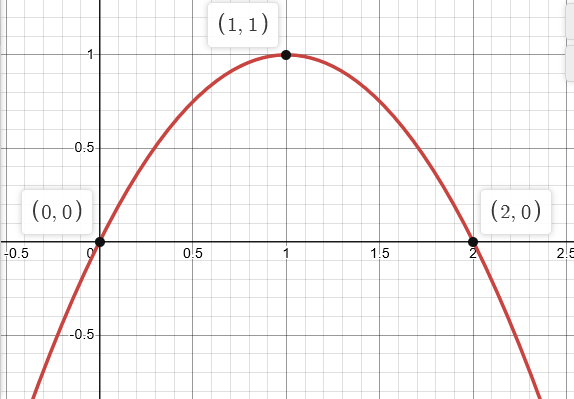
\includegraphics[scale=0.5]{66.png}\\

\next
68.\begin{align}
    \set
    f(0)&=f(2)=0\\
    f'(x)&<0,\,\,\,\, x<1\\
    f'(1)&=0\\
    f'(x)&>0,\,\,\,\,x>1\\
    f''(x)&>0
\end{align}
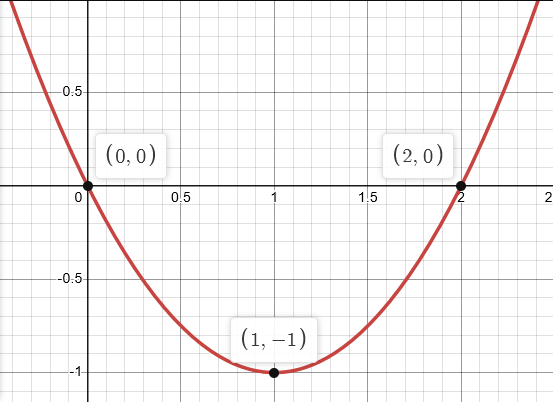
\includegraphics[scale=0.5]{68.png}

\section{Capstone}
70. Water is running into the vase shown in the figure at a constant rate.\\
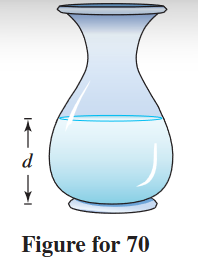
\includegraphics{70a.png}\\
(a) Graph the depth $d$ of water in the vase as a function of time.\\
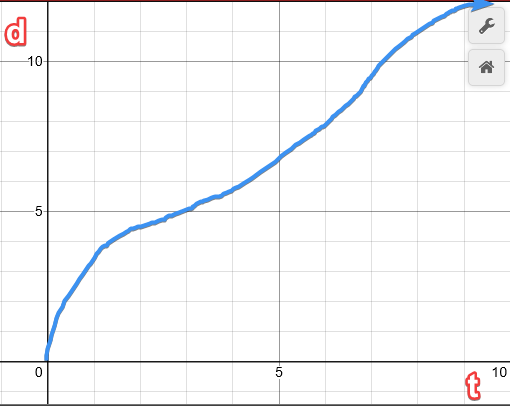
\includegraphics[scale=0.5]{70b.png}\\
(b) Does the function have any extrema? Explain.\\
\indent There are no relative extrema since the depth is always increasing.\\
\next
(c) Interpret the inflection points of the graph of $d$.\\
\indent The rate of changes $d$ decreases until the liquid reaches the vase's widest point, then the rate increases in the vase's narrowest point, and the rate decreases again when the top of vase is reached.\\

\section{Find $a, b, c,$ and $d$ such that the cubic $f(x)=ax^3+bx^2+cx+d$ satisfies the given conditions.}
74.\begin{enumerate}
    \item Relative maximum: (2, 4)
    \item Relative minimum: (4, 2)
    \item Inflection point (3, 3)
\end{enumerate}
\begin{align}
    \set
    f'(x)&=3ax^2+2bx+c\\
    f''(x)&=6ax+2b\\
    f(2)&=8a+4b+2c+d=4\\
    f(3)&=64a+16b+4c+d=2
\end{align}
By equations 3 and 4, it follows that:
\begin{align}
    56a+12b+2c&=-2\\
    28a+6b+c&=-1\\
    f'(2)=12a+4b+c&=0\\
    f'(4)=48a+8b+c&=0\\
    f''(3)=18a+2b&=0
\end{align}
We have that
\begin{align}
    18a+2b&=0\\
    16a+2b&=-1\\
    2a&=1
\end{align}
and
\begin{align}
    28a+6b+c&=1\\
    12a+4b+c&=0\\
    16a+2b&=-1
\end{align}
Therefore,
\begin{align}
    a&=\frac{1}{2}\\
    b&=-\frac{9}{2}\\
    c&=12\\
    d&=-6\\
    f(x)&=\frac{1}{2}x^3-\frac{9}{2}x^2+12x-6
\end{align}

\section{Word problems}
74. The total cost $C$ of ordering and storing $x$ units is $C=2x+\frac{300000}{x}$. What order size will produce a minimum cost?
\begin{align}
    \set
    C'&=2-\frac{300000}{x^2}\\
    &=0\,\,\text{when}\,\, x=100\sqrt[]{15}=387
\end{align}
An order size of 387 units will produce a minimum cost.\\

\next
82. The average typing speed $S$ (in words per minute) of a typing student after $t$ weeks of lessons is shown in the table.\\
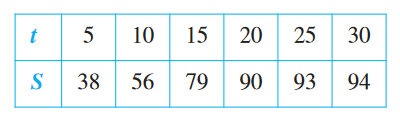
\includegraphics{82.png}\\
A model for the data is $S=\frac{100t^2}{65+t^2},\,\,\, t>0$.\\
(b) Use the second deritvative to determine the concavity of $S$. Compare the result with the graph in part (a).
\begin{align}
    \set
    S'(t)&=\frac{13000}{(65+t^2)^2}\\
    S''(t)&=\frac{13000(65-3t^2)}{(65+t^2)}=0\\
    t&=4.65
\end{align}
S is concave upwards on (0, 4.65) and downwards on (4.65, 30).\\

\vs
\next
(c) What is the sign of the first derivative for $t>0$? By combining this information with the concavity of the model, what inferences can be made about the typing speed as $t$ increases.\\
\[S'(t)>0,\,\,\,\, t>0\]
The speed increases at a slower rate as $t$ increases.

\vs
\next
88. Show that the point of inflection of $f(x)=x(x-6)^2$ lies midway between the relative extrema of $f$.
\begin{align}
    \set
    f(x)&=x(x-6)^2\\
    &=x^3-12x^2+36x\\
    f'(x)&=3x^2-24x+36\\
    &=3(x-2)(x-6)\\
    &=0\\
    f''(x)&=6x-24\\
    &=6(x-4)=0
\end{align}
(6, 0) and (2, 32) are relative extrema.
(4, 16) is the point of inflection, and it lies midway between $f$'s relative extrema.

\section{Determine whether the statement is true or false. If it is false, explain why or give an example that shows it is false.}
91. The graph of every cubic polynomial has precisely one point of inflection.\\
\indent True.

\newpage \next
92. The graph of $f(x)=\frac{1}{x}$ is concave downward for $x<0$ and concave upward for $x>0$, and thus it has a point of inflection at $x=0$\\
\indent False. $f(x)$ is discontinuous at $x=0$.

\vspace{0.75cm}
\next
93. If $f'(c)>0$, then $f$ is concave upward at $x=c$\\
\indent False. Concavity is identified with $f''$. If $f(x)=x$ and $c=2$, $f$ will not be concave upward at $c=2$ even though $f'(c)=f(2)>0$.

\vspace{0.75cm}
\next
94. If $f''(2)$=0, then the graph of $f$ must have a point of inflection at $x=2$\\
\indent False. $f(x)=(x-2)^4$ doesn't have one.






































\end{document}